\chapter{HASIL DAN PEMBAHASAN}

Dalam bab ini dibahas mengenai hasil perbandingan dari pengukuran
partikel berbasis Dynamic Light Scattering dengan menggunakan
PSA, DLS sederhana dengan laser merah dan hijau.

\section{Hasil Pengujian Blok OPT101}
Fotodioda yang digunakan dalam penelitian ini merupakan OPT101
yang di dalamnya sudah terkombinasi dengan \textit{transimpedance
amplifier} dalam satu chip nya sehingga mengurangi error yang
bersumber dari kebocoran arus. Oleh karena itu pengujian blok
hanya bisa dilakukan dengan memanfaatkan langsung fotodioda
sebagai input arus. Sebagai komparasi maka digunakan resistor
dengan nilai 1M${\Omega}$, 2M${\Omega}$, 3M${\Omega}$, 
4M${\Omega}$, 5M${\Omega}$, 10M${\Omega}$ dan untuk perubahan 
arus yang akan masuk digunakan LED yang input DC nya terhubung 
dengan power supply agar nilai Voltasenya dapat diatur untuk 
merubah intensitas cahaya dari LED. 

\begin{figure}[H]
  \centering
  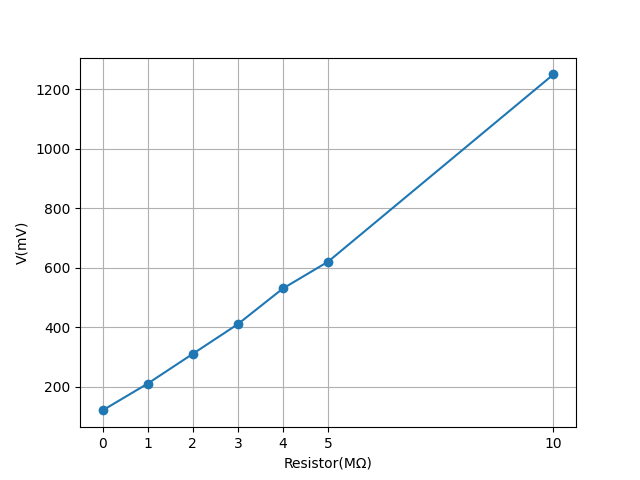
\includegraphics[width=12cm]{Images/Gain1.png}
  \caption{Nilai Output OPT101 terhadap Resistor}
  \label{fig:gain_res}
\end{figure}

Dari grafik diatas pembesaran nilai tegangan keluaran yang
dihasilkan dari rangkaian OPT101 menunjukan hasil yang linear
terhadap nilai resistor yang digunakan. IC yang tidak terhubung
dengan resistor memiliki nilai keluaran ${120mV}$, namun nilai
tersebut merupakan hasil yang ter invert sebelum melewati
rangkaian inverting sehingga perubahan nilai pada saat gelap
lebih tinggi dibandingkan saat lebih terang. Setelah diberikan
resistor secara inverting pada skema rangkaian \textit{Transimpedance
Amplifier}, nilai pembesaran yang diukur dengan menggunakan
persamaan:

\begin{equation}
  A_v = \frac{V_{output}}{V_{input}}
\end{equation}

didapatkan nilai 1,75 pada resistor 1M${\Omega}$, 2,58 pada
resistor 2M${\Omega}$, 3,41 pada resistor 3M${\Omega}$, 4,41
pada resistor 4M${\Omega}$, 5,16 pada resistor 5M${\Omega}$,
dan 10,41 pada resistor 10M${\Omega}$.

Untuk memastikan bahwa OPT101 mendeteksi perbedaan intensitas
cahaya maka dilakukan pengujian dengan memvariasikan intensitas
cahaya LED yang diletakan di depan fotodioda sehingga dihasilkan
data sebagai berikut

\begin{figure}[H]
  \centering
  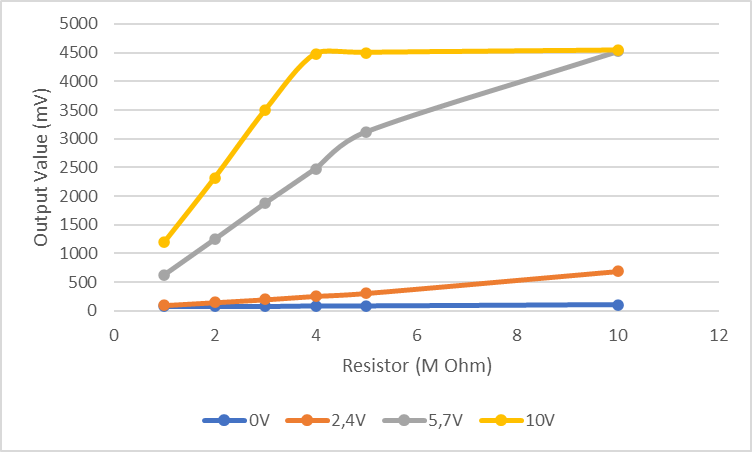
\includegraphics{Images/GainWLED.png}
  \caption{Nilai Output OPT101 terhadap Resistor}
  \vspace*{1.75pt}
  \caption*{dengan Variasi LED berbeda Intensitas Cahaya}
  \label{fig:gain_led}
\end{figure}

Pada saat LED tidak diberikan tegangan, keluaran dari OPT101 di
semua ukuran resistor hampir berdekatan pada kisaran ${70mV}$
hingga ${110mV}$. Ketika LED diberikan tegangan ${2,4V}$,
keluaran dari OPT101 pada setiap ukuran resistor memiliki
peningkatan sesuai gain oleh ukuran resistornya. LED yang
diberikan tegangan ${5,7V}$ dan ${10V}$ memiliki intensitas
cahaya yang lebih tinggi, namun data menunjukan adanya nilai
maksimum yang dibatasi oleh fotodiodanya. Output Value yang
dihasilkan dari OPT101 hanya dibatasi hingga nilai ${4500mV}$
sehingga pembesaran yang melebihi nilai ${4500mV}$ akan memiliki
nilai yang menyerupai nilai maksimum tersebut.

\section{Hasil Pengujian Instrumen Dynamic Light Scattering}
Kedua rangkaian alat yang digunakan merupakan modul rangkaian
dengan laser yang berbeda. Satu rangkaian menggunakan laser
merah dan rangkaian lainnya menggunakan laser hijau. Pada
pengujian ini digunakan sampel ${SiO_2}$ dengan pelarut aquades.

\subsection{Data Fluktuasi Sinyal}
Untuk memastikan kesesuaian data dari setiap pengukuran, maka
dilakukan beberapa pengukuran untuk membandingkan distribusi
persebaran ukuran partikel setiap waktunya dari masing-masing
laser.

\begin{figure}[H]
  \noindent
  \centering
  \begin{longtable}{p{7cm}p{7cm}}
    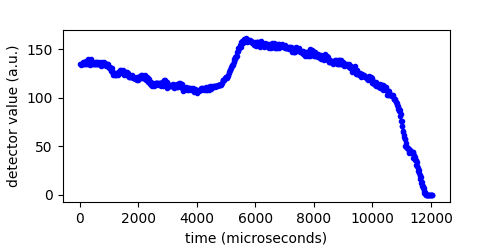
\includegraphics[width=8cm]{Images/RawData_Hijau_Data10-01.png}
    &
    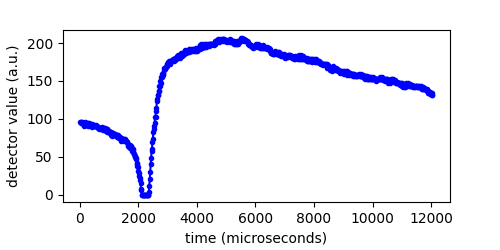
\includegraphics[width=8cm]{Images/RawData_Merah_Data9-01.png} \\
    
    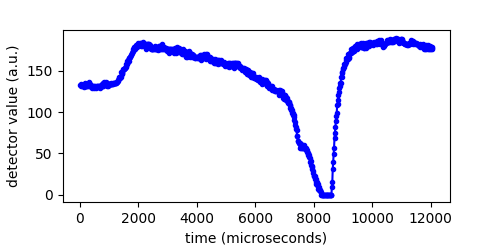
\includegraphics[width=8cm]{Images/RawData_Hijau_Data100-01.png}
    &
    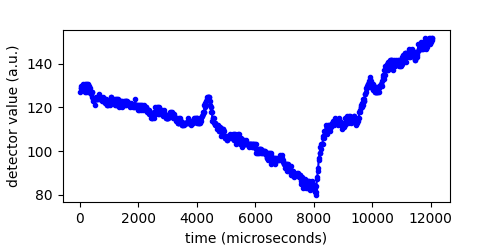
\includegraphics[width=8cm]{Images/RawData_Merah_Data99-01.png} \\
   
  \end{longtable}
\end{figure}
\begin{figure}
  \ContinuedFloat
  \begin{longtable}{p{7cm}p{7cm}}
    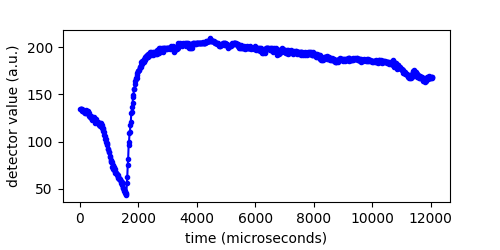
\includegraphics[width=8cm]{Images/RawData_Hijau_Data1000-01.png}
    \centering{Laser Hijau}
    &
    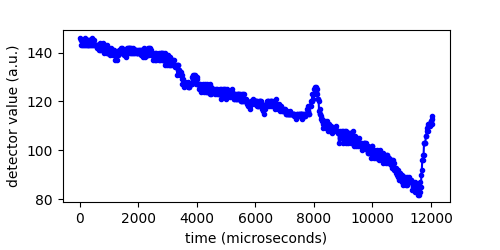
\includegraphics[width=8cm]{Images/RawData_Merah_Data1000-01.png} 
    \centering{Laser Merah}\\
  \end{longtable}

  \caption{Sampel Nilai Detektor Sensor terhadap Waktu}
\end{figure}

Grafik diatas menunjukkan beberapa data fluktuasi yang diukur
melalui 10.000 pengulangan dengan 800 nilai pada setiap
pengulangan dalam durasi 12.048 mikrodetik pada masing-masing
laser. Melalui grafik dapat dilihat bahwa fluktuasi yang
dihasilkan berbeda pada masing-masing laser, data yang terbaca
oleh sensor dari hamburan partikel menggunakan laser hijau
memiliki pola fluktuasi yang lebih bervariasi dibandingkan
dengan laser merah yang seringkali tidak mendeteksi perubahan
yang signifikan. Pada rangkaian laser merah  fluktuasi yang
dihasilkan memiliki pola yang hampir serupa pada setiap
pengukurannya.

Selain itu melalui grafik juga dapat diketahui bahwa hamburan
dari laser hijau memiliki fluktuasi yang cukup cepat, dapat
diperlihatkan dari seberapa cepat detektor mencapai lembah dan
kembali lagi ke puncak, sedangkan hamburan dari laser merah
dominan memiliki perubahan yang lebih lambat.

\subsection{Data Autokorelasi}
Fluktuasi nilai dari sensor pada setiap pengukurannya dapat
dijadikan acuan sebagai seberapa cepat partikel tersebut
bergerak. Untuk mendapatkan nilai ukuran partikel diperlukan
nilai autokorelasi yang merupakan korelasi dari setiap nilai
pada setiap pengulangan. Nilai autokorelasi didapatkan dengan
menggunakan \textit{library Numpy} dari Python untuk mempermudah
pengolahan data berbentuk matriks. Dari nilai autokorelasi
terebut dapat di plotting menjadi gambar berikut:

\begin{figure}[H]
  \noindent
  \centering
  \begin{longtable}{p{7cm}p{7cm}}
    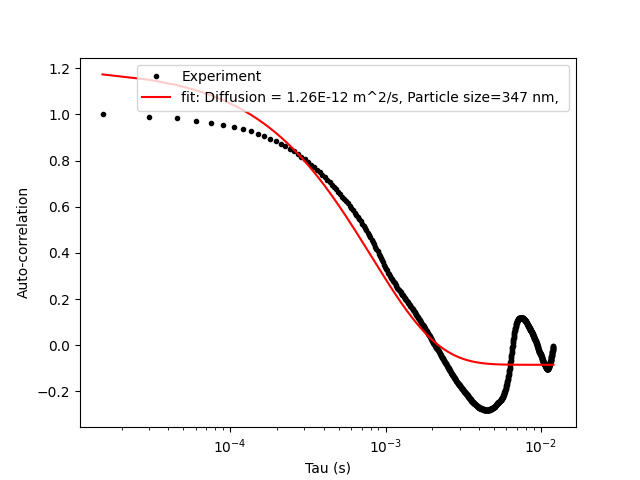
\includegraphics[width=8cm]{Images/AutoCor_Hijau_Data10-01.png}
    &
    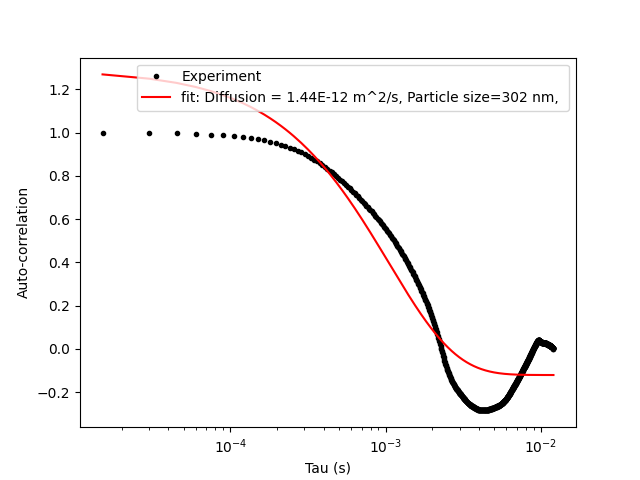
\includegraphics[width=8cm]{Images/AutoCor_Merah_Data9-01.png} \\
    
    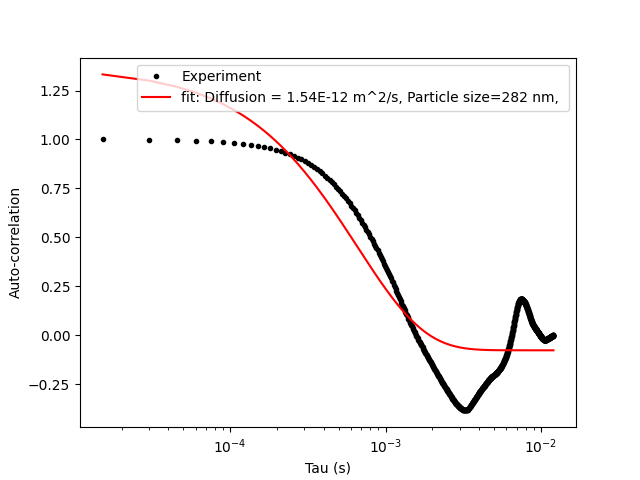
\includegraphics[width=8cm]{Images/AutoCor_Hijau_Data100-01.png}
    &
    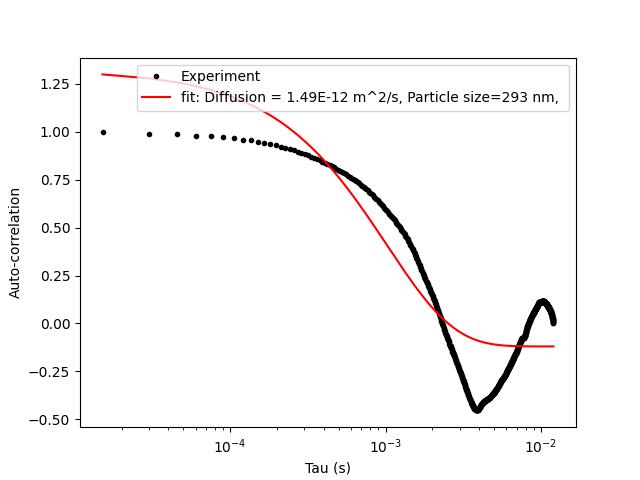
\includegraphics[width=8cm]{Images/AutoCor_Merah_Data99-01.png} \\
   
  \end{longtable}
\end{figure}
\begin{figure}
  \ContinuedFloat
  \begin{longtable}{p{7cm}p{7cm}}
    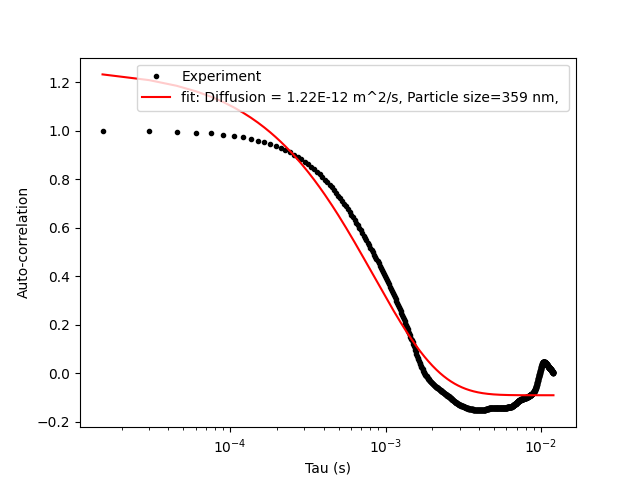
\includegraphics[width=8cm]{Images/AutoCor_Hijau_Data1000-01.png}
    \centering{Laser Hijau}
    &
    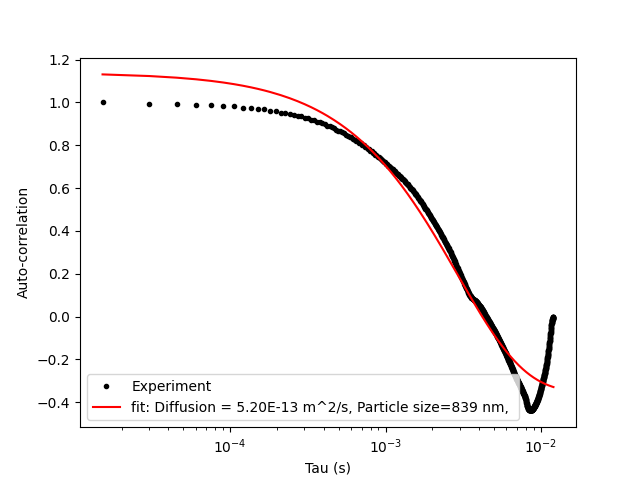
\includegraphics[width=8cm]{Images/AutoCor_Merah_Data1000-01.png} 
    \centering{Laser Merah}\\
  \end{longtable}

  \caption{Sampel Data Autokorelasi terhadap Tau}
\end{figure}

\subsection{Distribusi Data Ukuran Partikel}
\begin{figure}[H]
  \centering
  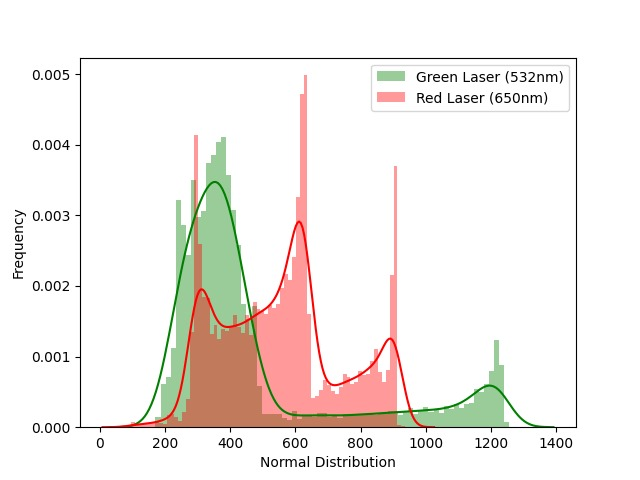
\includegraphics[width=13cm]{Images/Distribusi 1000x.jpg}
  \caption{Distribusi 10000 Ukuran Partikel}
  \label{fig:dist10000x}
\end{figure}

Grafik diatas merupakan grafik distribusi frekuensi terhadap
diameter dari partikel. Distribusi kedua data dengan 10.000
iterasi pada masing-masing laser memiliki perbedaan hasil
kumulatif yang cukup signifikan. Persebaran diameter partikel
dengan laser merah memiliki range yang lebar dengan beberapa
puncak, seperti yang terlihat pada grafik dimana diameter
partikel memiliki puncak pada rentang ${300nm-350nm}$ dan
${580nm-620nm}$. Adanya tiga puncak dari grafik distribusi diatas
menunjukan adanya tiga ukuran partikel yang terdeteksi. Perubahan
nilai pada sensor yang lambat menghasilkan perhitungan dimeter
partikel yang lebih besar, namun terdapat beberapa pengulangan
yang mendeteksi perubahan dengan cepat sehingga dapat mengukur
diameter partikel yang lebih kecil. Berbeda dengan laser hijau
yang memiliki persebaran diameter partikel yang memiliki puncak
pada rentang ${200nm-400nm}$. Range data yang terukur pada laser
hijau dominan lebih kecil dibandingkan pada laser merah. Hal ini
menunjukan bahwa laser hijau dapat mendeteksi diameter partikel
yang lebih kecil dibandingkan denga laser merah.



\section{Hasil Pengujian Sampel pada PSA}
\begin{figure}[H]
  \centering
  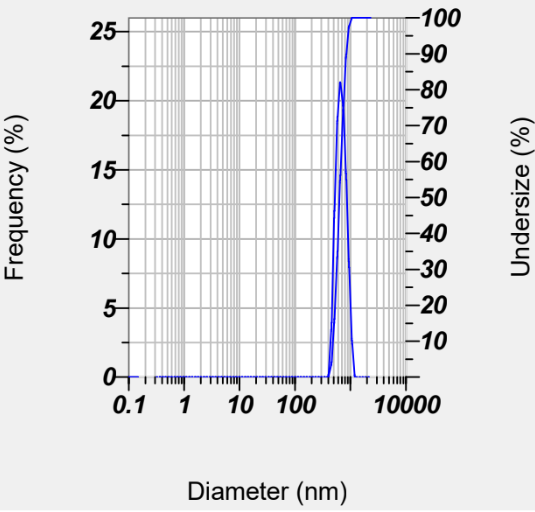
\includegraphics[width=10cm]{Images/SiO2PSA.png}
  \caption{Distribusi Ukuran Partikel pada PSA}
  \label{fig:psa}
\end{figure}
Pada pengukuran PSA, data yang didapat berupa ${Z-Average}$ berkisar
di ${463,1 nm}$ dengan PI 2,592. Data tersebut mempengaruhi pengukuran
dari PSA karena Polidyspersity Index yang tinggi mengurangi tingkat
akurasi pada pengukuran. Apabila dibandingkan dengan kedua rangkaian
DLS yang diuji, distribusi data diameter partikel yang didapat
memiliki range lebih sempit. Lebar range tersebut juga mempengaruhi
tingkat akurasi dari pengukuran pada rangkaian yang digunakan.



% \section{Gambar}

% \begin{figure}[H]
%   \centering
%   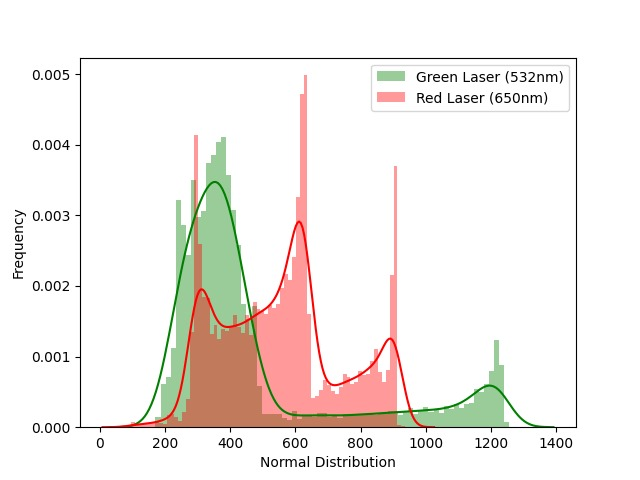
\includegraphics[width=8cm]{Images/Distribusi 1000x.jpg}
%   \caption{Contoh Gambar}
%   \label{fig:blg}
% \end{figure}

% \begin{enumerate}
%   \item Gambar dimuat kira-kira di tengah-tengah halaman.
%   \item Judulnya ditik di bawah gambar, mengikuti lebar gambar dengan memperhitungkan keseimbangan halaman.
%   \item Nomor gambar terdiri atas dua bagian, yaitu:
%   \begin{enumerate}[label=(\alph*)]
%     \item bagian pertama menunjukkan nomor bab tempat gambar itu dimuat;
%     \item bagian kedua menunjukkan nomor urut gambar pada bab itu. Misalnya, Gambar  \ref{fig:blg} menunjukkan bahwa gambar itu ada pada Bab IV dan merupakan gambar urutan pertama pada bab itu.
%   \end{enumerate}
%   \item Kalimat pertama judul gambar ditulis dengan jarak dua ketukan sesudah nomor gambar.
%   \item Awal baris kedua judul gambar berada di bawah awal judul gambar (bukan di bawah nomor gambar).
% \end{enumerate}

% \section{Grafik}
% \begin{figure}[H]
%   \begin{subfigure}{.5\textwidth}
%     \centering
%     \includegraphics[width=6.7cm]{Gambar/cv.pdf}
%   \end{subfigure}
%   \hspace{0.7em}
%   \begin{subfigure}{.5\textwidth}
%     \centering
%     \includegraphics[width=6.7cm]{Gambar/cv_comp.pdf}
%   \end{subfigure}
%   \caption{Contoh Grafik}
%   \label{fig:cv}
%   \end{figure}

% \begin{enumerate}
%   \item Grafik dimuat kira-kira di tengah-tengah halaman.
%   \item Judulnya ditik di atas grafik, mengikuti lebar grafik, dengan memperhitungkan keseimbangan halaman.
%   \item Nomor grafik terdiri atas dua bagian, yaitu:
%   \begin{enumerate}[label=(\alph*)]
%     \item bagian pertama menunjukkan nomor bab grafik itu dimuat; 
%     \item bagian kedua menunjukkan nomor urut grafik pada bab itu. Misalnya, Gambar  ~\ref{fig:cv} menunjukkan bahwa grafik itu ada pada Bab IV dan merupakan grafik urutan keempat pada bab itu.
%   \end{enumerate}
%   \item Kalimat pertama judul grafik ditulis dengan jarak dua ketukan sesudah nomor grafik.
%   \item Awal baris kedua judul grafik berada di bawah awal judul grafik (bukan di bawah nomor grafik).
% \end{enumerate}

% \section{Tabel}
% \begin{table}[ht!]
%   \centering
%   \caption{Contoh Tabel}
%   \begin{tabular}{|l|l|l|l|l|l|}
%   \hline
%   \textbf{Sistem} & \textbf{m, n} & \textbf{\begin{tabular}[c]{@{}l@{}}Sudut\\ Puntir (\degree)\end{tabular}} & \textbf{\begin{tabular}[c]{@{}l@{}}Duplikasi\\ ($x \times y \times z$)\end{tabular}} & \textbf{\begin{tabular}[c]{@{}l@{}}Panjang\\ Sistem (\AA)\end{tabular}} & \textbf{\begin{tabular}[c]{@{}l@{}}Jumlah\\ Atom\end{tabular}} \\ \hline
%   SLG             & -             & -                                                                  & 1 x 1 x 1                                                                & 35,98                                                                 & 434                                                            \\ \hline
%   BLG          & -             & 0                                                                  & 1 x 1 x 1                                                                & 35,98                                                                 & 868                                                            \\ \hline
%   tBLG            & 9, 8          & 3,89                                                               & 1 x 1 x 1                                                                & 35,98                                                                 & 868                                                            \\ \hline
%   tBLG            & 8, 7          & 4,41                                                               & 1 x 1 x 1                                                                & 31,75                                                                 & 676                                                            \\ \hline
%   tBLG            & 5, 3          & 16,43                                                              & 2 x 2 x 1                                                                & 34,20                                                                  & 784                                                            \\ \hline
%   \end{tabular}
%   \label{tab:str}
%   \end{table}

% \begin{enumerate}
%   \item Tabel dimuat kira–kira di tengah–tengah halaman.
%   \item Judulnya ditik di atas tabel, mengikuti lebar tabel, dengan memperhitungkan keseimbangan halaman.
%   \item Nomor tabel terdiri atas dua bagian, yaitu:
%   \begin{enumerate}[label=(\alph*)]
%     \item bagian pertama menunjukkan nomor bab tabel itu dimuat;
%     \item bagian kedua menunjukkan nomor urut tabel pada bab itu. Misalnya, Tabel ~\ref{tab:str} menunjukkan bahwa tabel itu berada pada Bab IV dan merupakan tabel urutan pertama pada bab itu.
%   \end{enumerate}
%   \item Kalimat pertama judul tabel ditulis dengan jarak dua ketukan sesudah nomor tabel.
%   \item Awal baris kedua judul tabel berada di bawah awal judul tabel (bukan di bawah nomor tabel).
%   \item Ukuran huruf pada isi tabel adalah 10 pt.
%   \item Isi tabel ditulis dalam 1 spasi.
% \end{enumerate}

% \section{Persamaan}

% \begin{equation}
%   U_{i j}^{\mathrm{LJ}}\left(r_{i j}\right)=4 \epsilon_{i j}\left[\left(\frac{\sigma_{i j}}{r_{i j}}\right)^{12}-\left(\frac{\sigma_{i j}}{r_{i j}}\right)^{6}\right]
% \end{equation}

% \begin{equation}
%   f_{Q}=\frac{C_v(T)}{3Nk_B}=\frac{\displaystyle\int\limits_{0}^{\infty}\frac{u^2e^u}{{(e^u-1)}^2}G(\omega)d\omega}{\displaystyle\int\limits_{0}^{\infty}G(\omega)d\omega}
% \end{equation}

% \section{Sitasi}
% Sitasi dapat dimasukkan seperti ini \cite{moore1998cramming}. Untuk sitasi dengan beberapa sumber, dapat dituliskan juga \cite{wang2020frank,zhang2020molecular}. Atau untuk tiga sumber seperti ini \cite{mcgaughey2019phonon,jiang2015graphene,khan2015equilibrium}.